\chapter{Physics Projections 2023-2025}
\label{chap:physics_projections}

In this Chapter we present a sampling of the key physics that sPHENIX will deliver with the run plan for 2023-2025 detailed in Chapter~\ref{chap:beam_use_proposal}.    

{\textcolor{red}{In this Chapter, we utilize projections based on the 28 cryo-week scenarios.   Tentative decision.}}

\section{Jet and Photon Physics}

\section{Heavy Flavor Physics}
\label{sec:HF}


\begin{figure}[htbp]
\centering
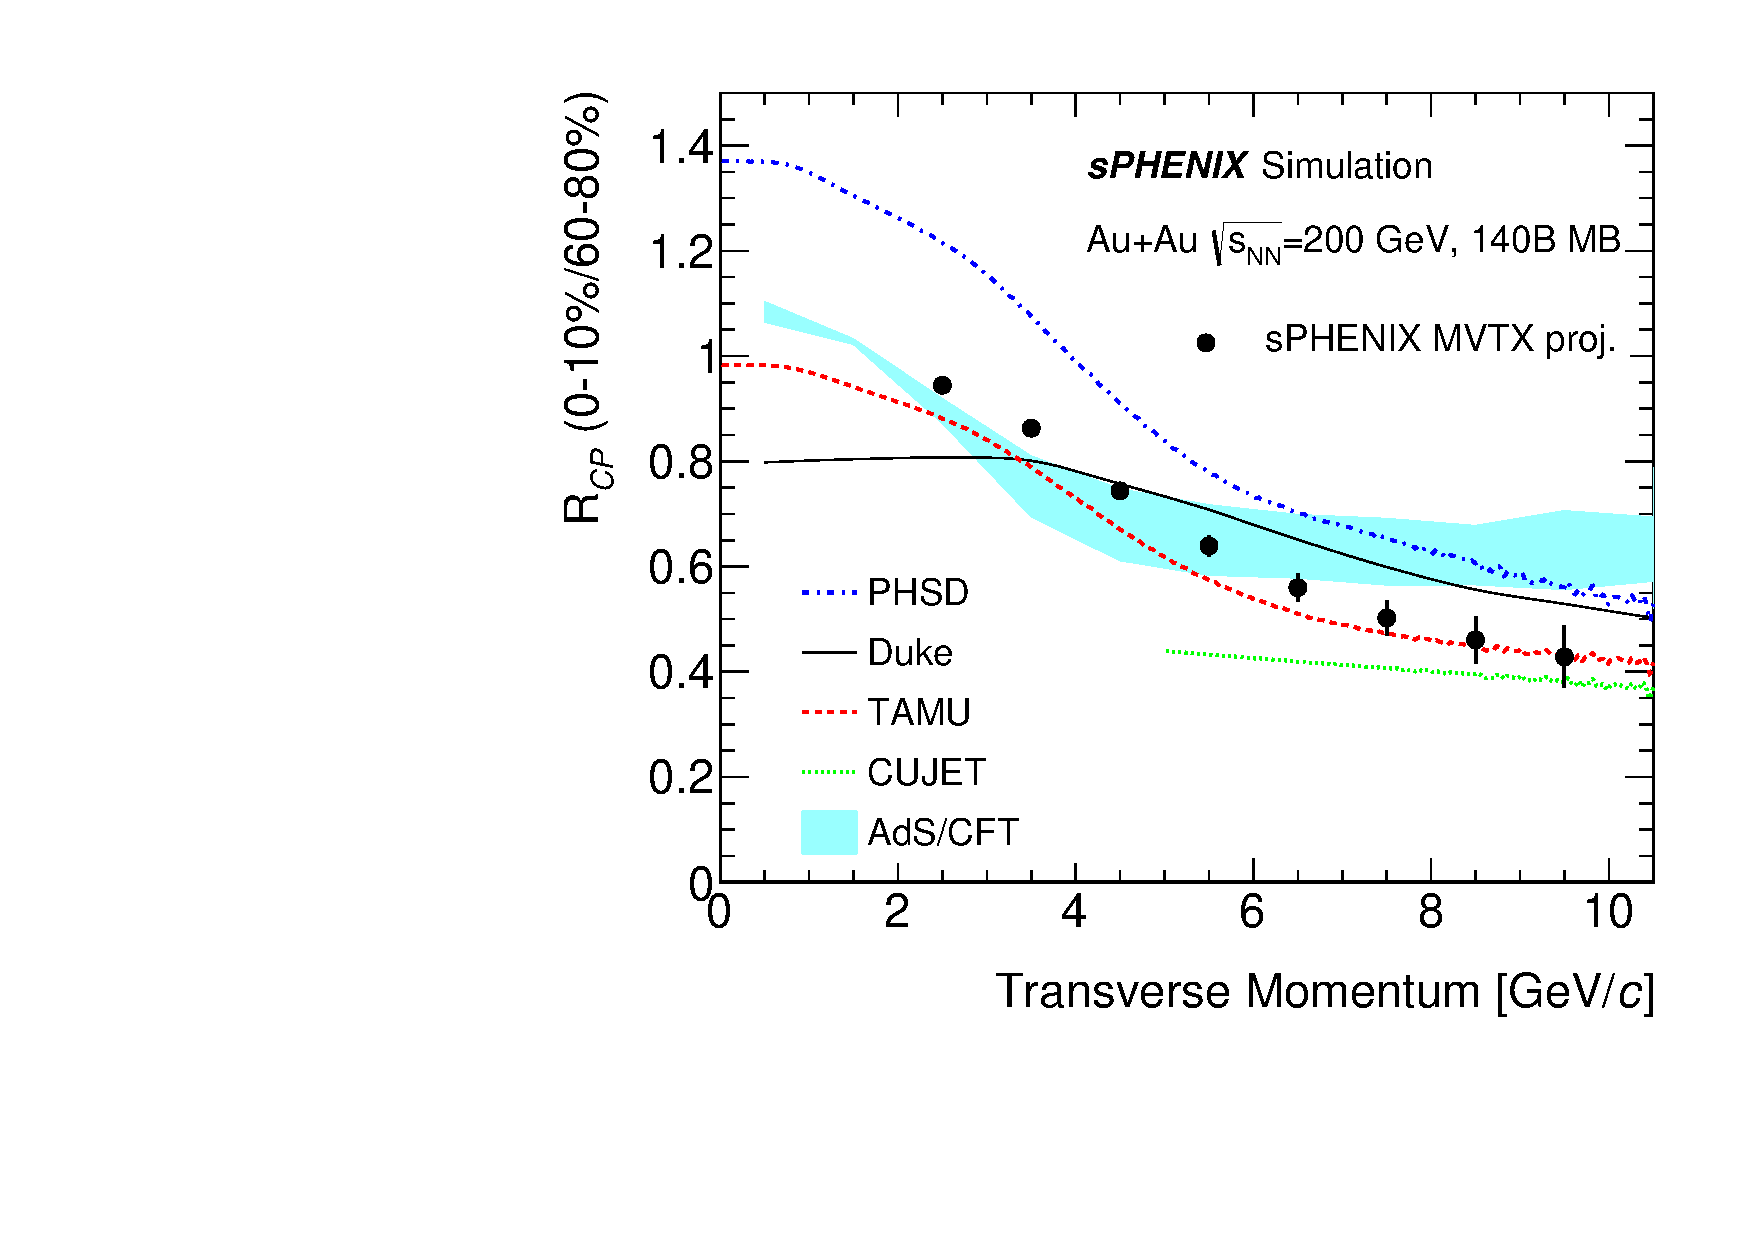
\includegraphics[width=0.48\textwidth]{figs/Rcp_proj_140B_theory.pdf}
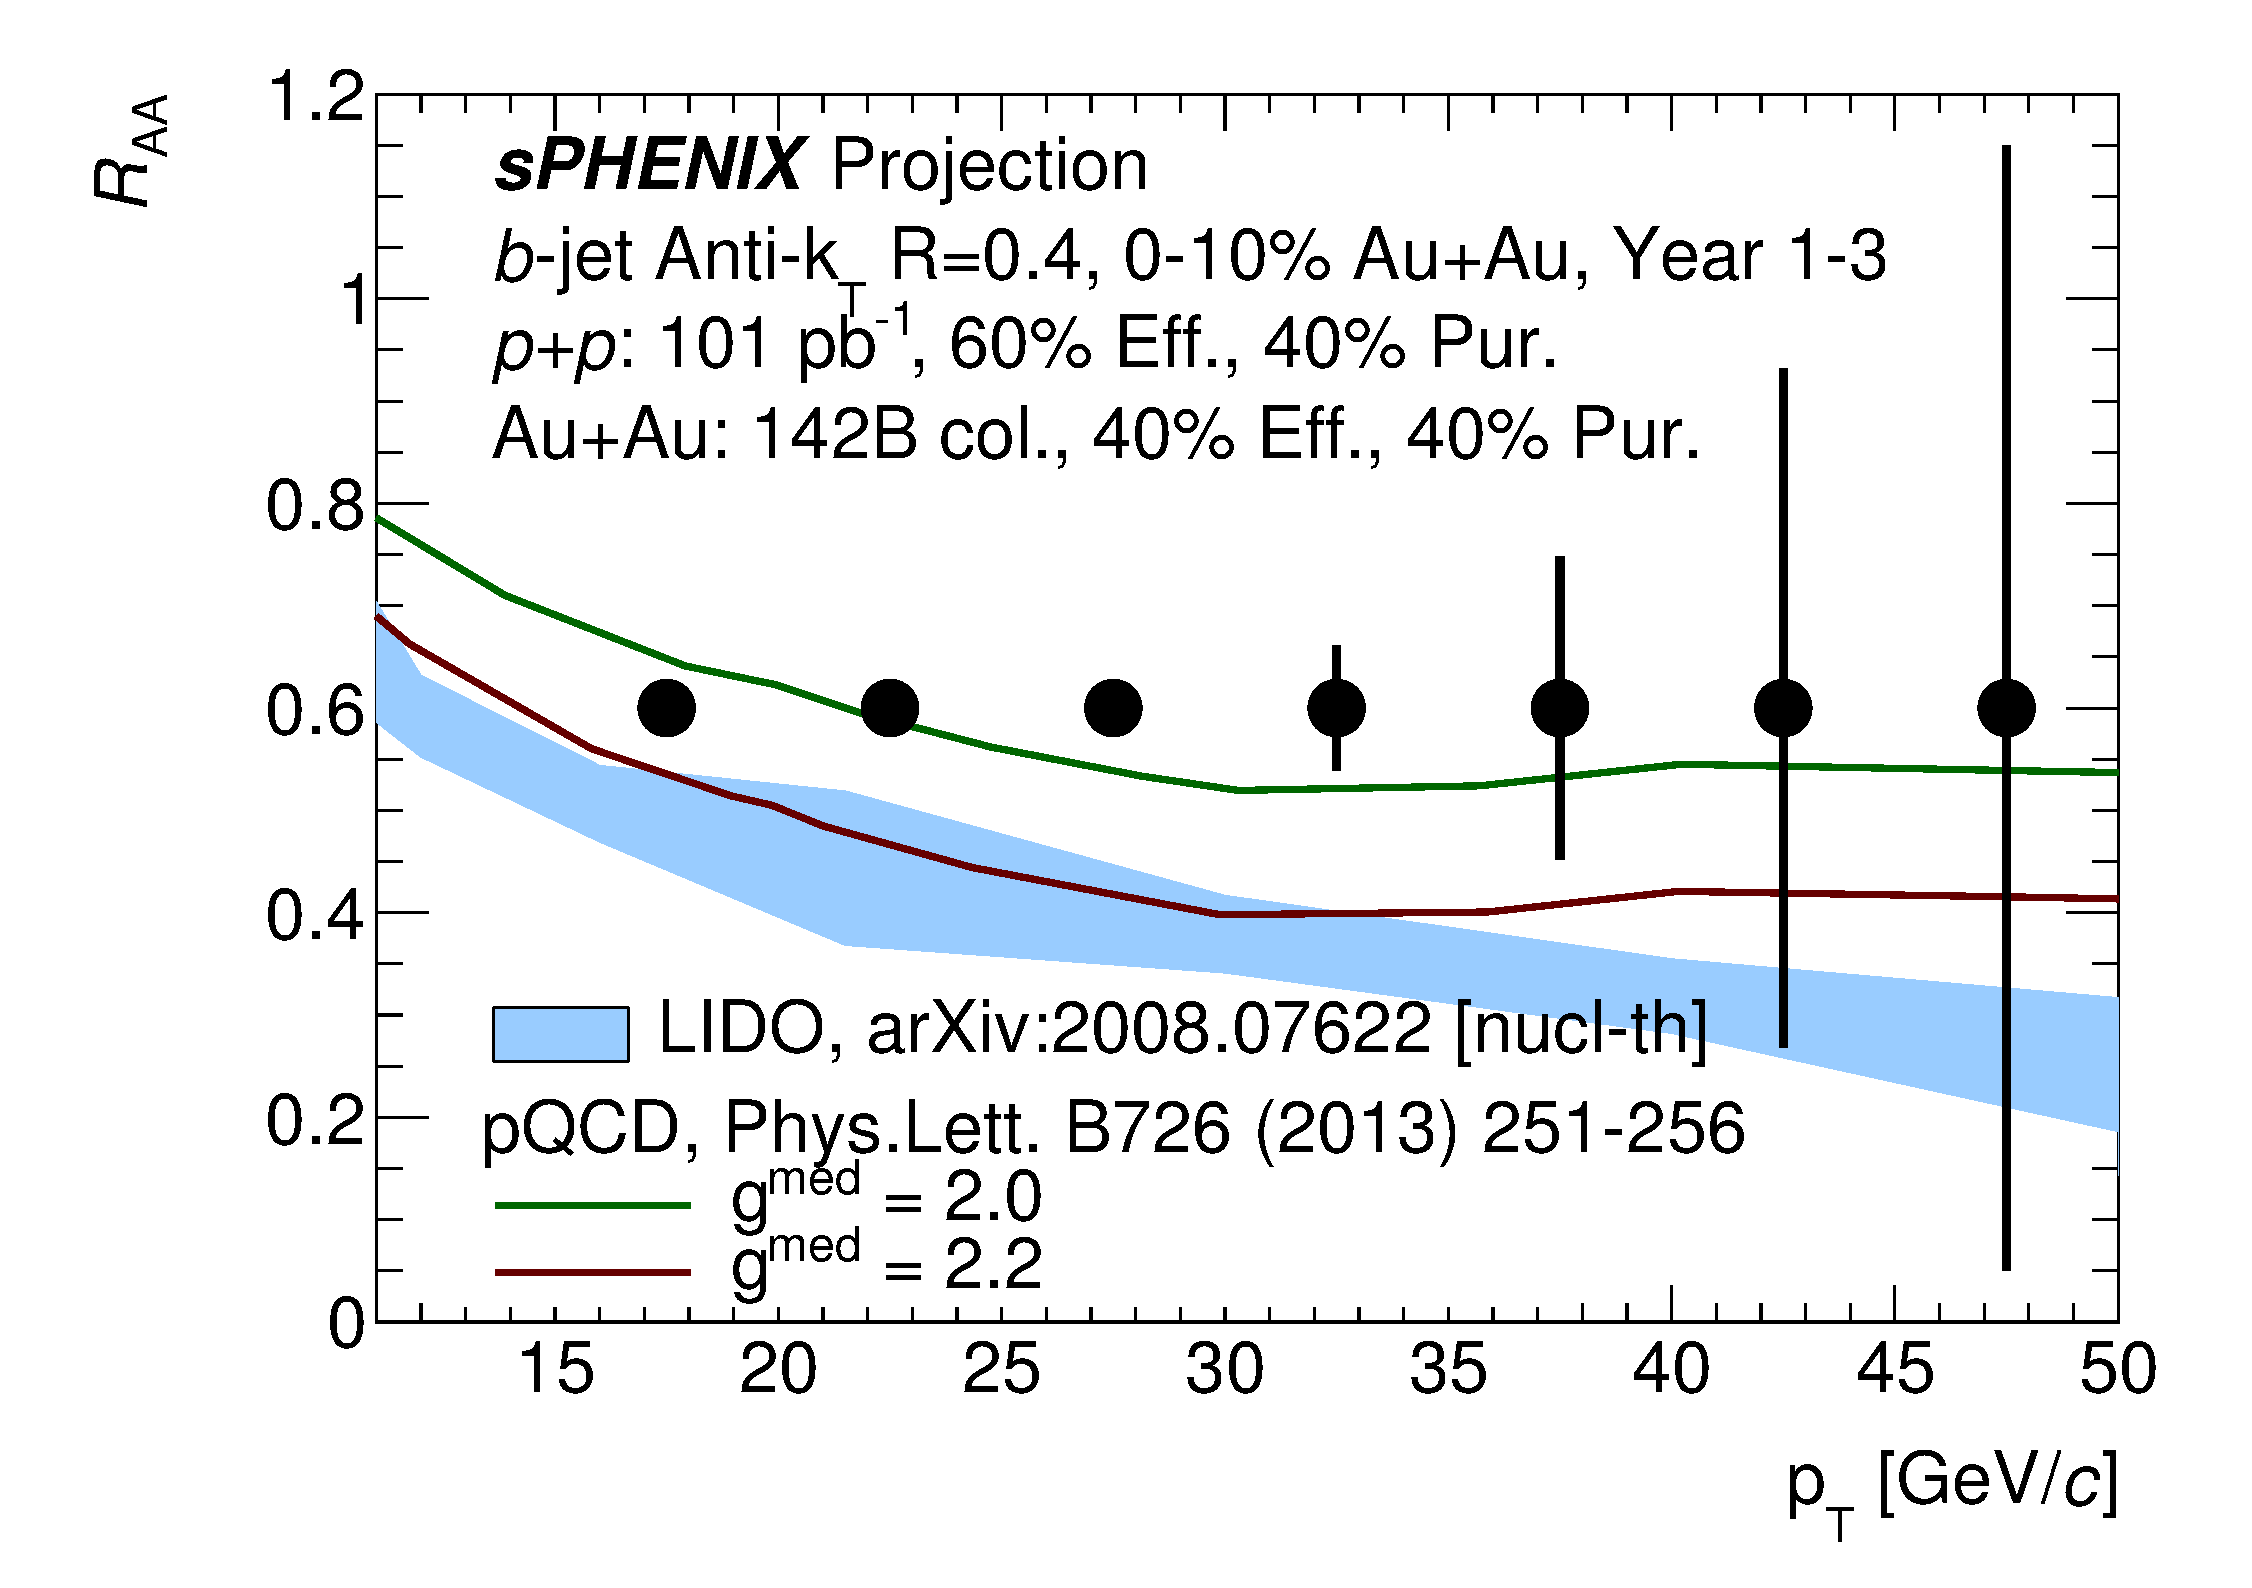
\includegraphics[width=0.5\textwidth]{figs/200pp_pythia8_CTEQ6L_7GeV_ALL_cfg_eneg_DSTReader_root_Draw_HFJetTruth_CrossSection2RAA_Theory_3yr_deta0_70.pdf}
\caption{Projected statistical uncertainties of nuclear modification factor $R_{cp}$ and \raa measurements of non-prompt/prompt $D^0$ mesons (left) and $b$-jet (right) as a function of \pT in 0--10\% central \auau collisions at $\sqrt{s_{NN}}=200$~GeV from a dataset of 140 billion minimum bias \auau collisions expected from the three-year sPHENIX operation. Left: the solid blue and red lines are best fit to the RHIC data, the solid black line is from a model calculation for B mesons and the dotted line is the theory calculation for $D$-mesons coming from $B$-meson decays. Right: the solid and dashed lines are from model calculations with two different coupling parameters to the QGP medium, $g^{\textrm{med}}$, and the statistical projection is based on the assumption of $\raa =0.6$. sPHENIX will enable these highest precision $B$-meson measurement and the first heavy flavor jet measurement at RHIC, which will place stringent tests on models describing the coupling between heavy quarks and the QGP~\cite{Huang:2013vaa,Duke,TAMU,PHSD,CUJET}}
\label{fig:HF-inclusive-RAA}
\end{figure}

\begin{figure}[htbp]
\centering
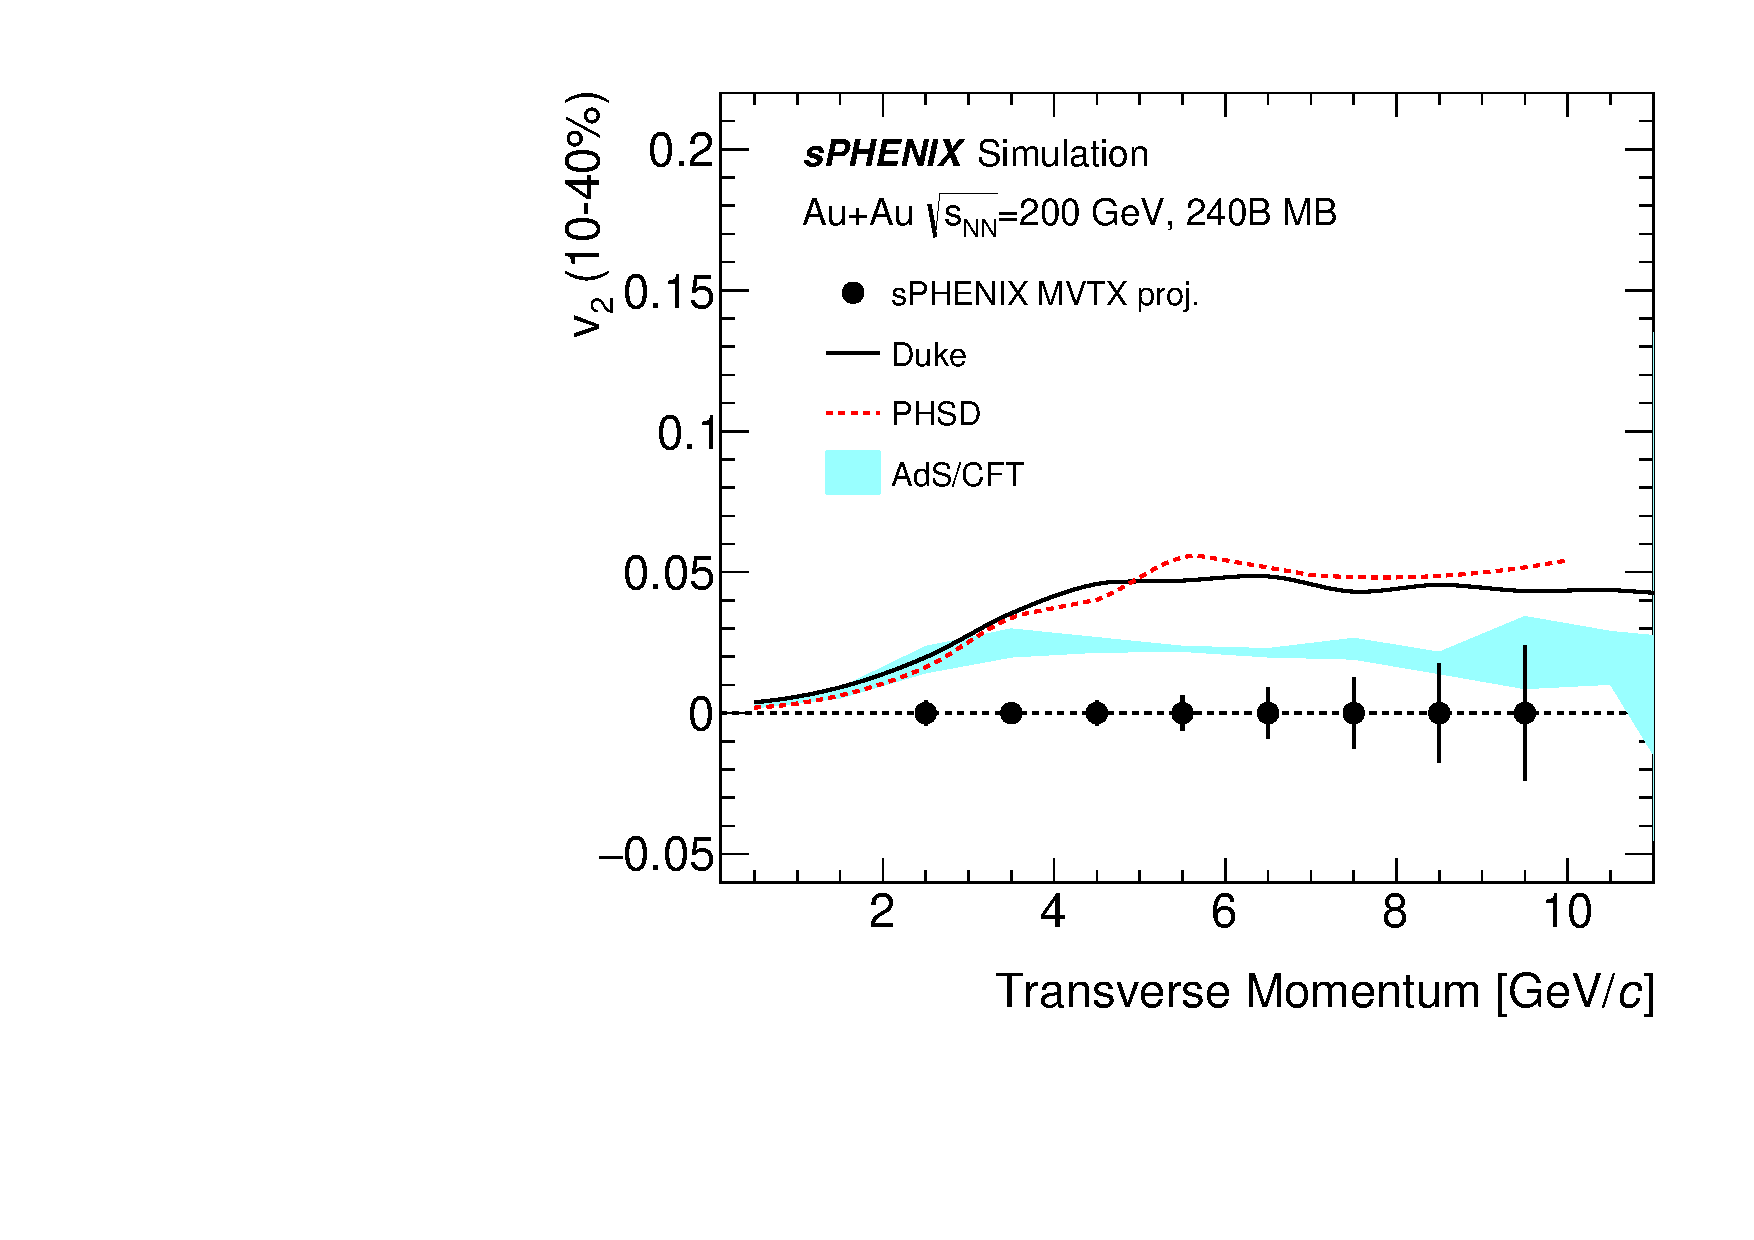
\includegraphics[width=0.48\textwidth]{figs/v2_proj_240B_theory.pdf}
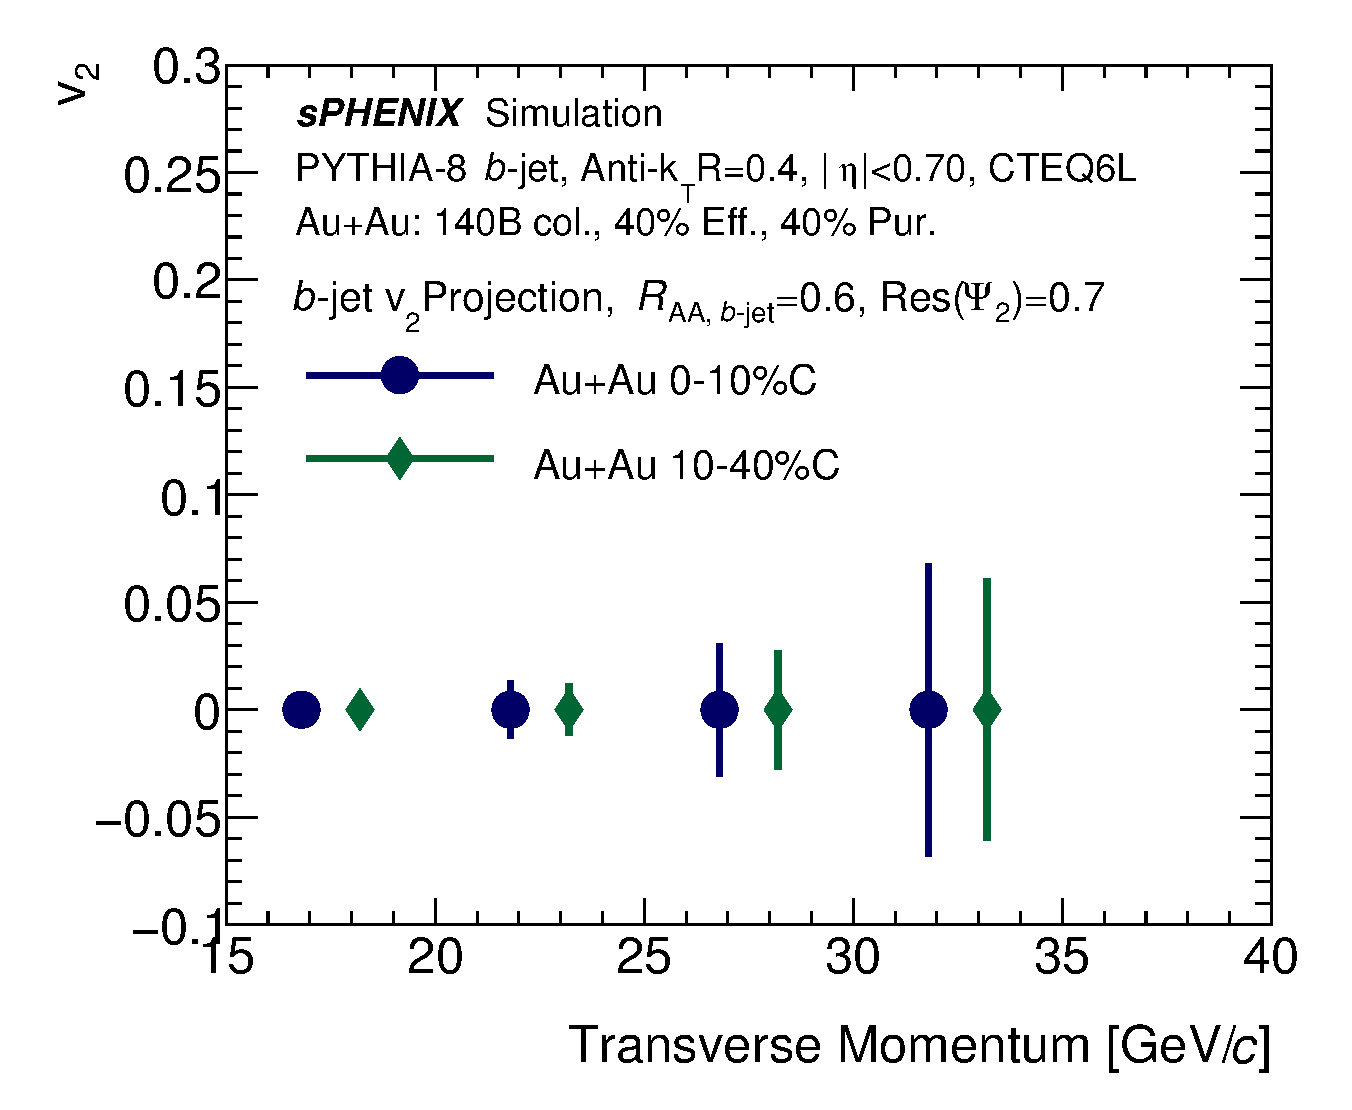
\includegraphics[width=0.5\textwidth]{figs/200pp_pythia8_CTEQ6L_7GeV_ALL_cfg_eneg_DSTReader_root_Draw_HFJetTruth_CrossSection2v2_3yr_EPR0_7_deta0_70.pdf}
\caption{Projected statistical uncertainties of $v_2$ measurements of non-prompt/prompt $D^0$ mesons (left) and $b$-jets (right) as a function of \pT in 10--40\% central \auau collisions at $\sqrt{s_{NN}}=200$~GeV from a dataset of 140 billion minimum bias \auau events expected from the three-year sPHENIX operation.  Left: the blue dotted line is from best fit of RHIC data, and the black line is for $B$-meson assuming $m_T$ scaling in $v_2$. \cite{Adamczyk:2017xur, Duke, TAMU, PHSD}}
\label{fig:HF-v2}
\end{figure}


\begin{figure}[htbp]
\centering
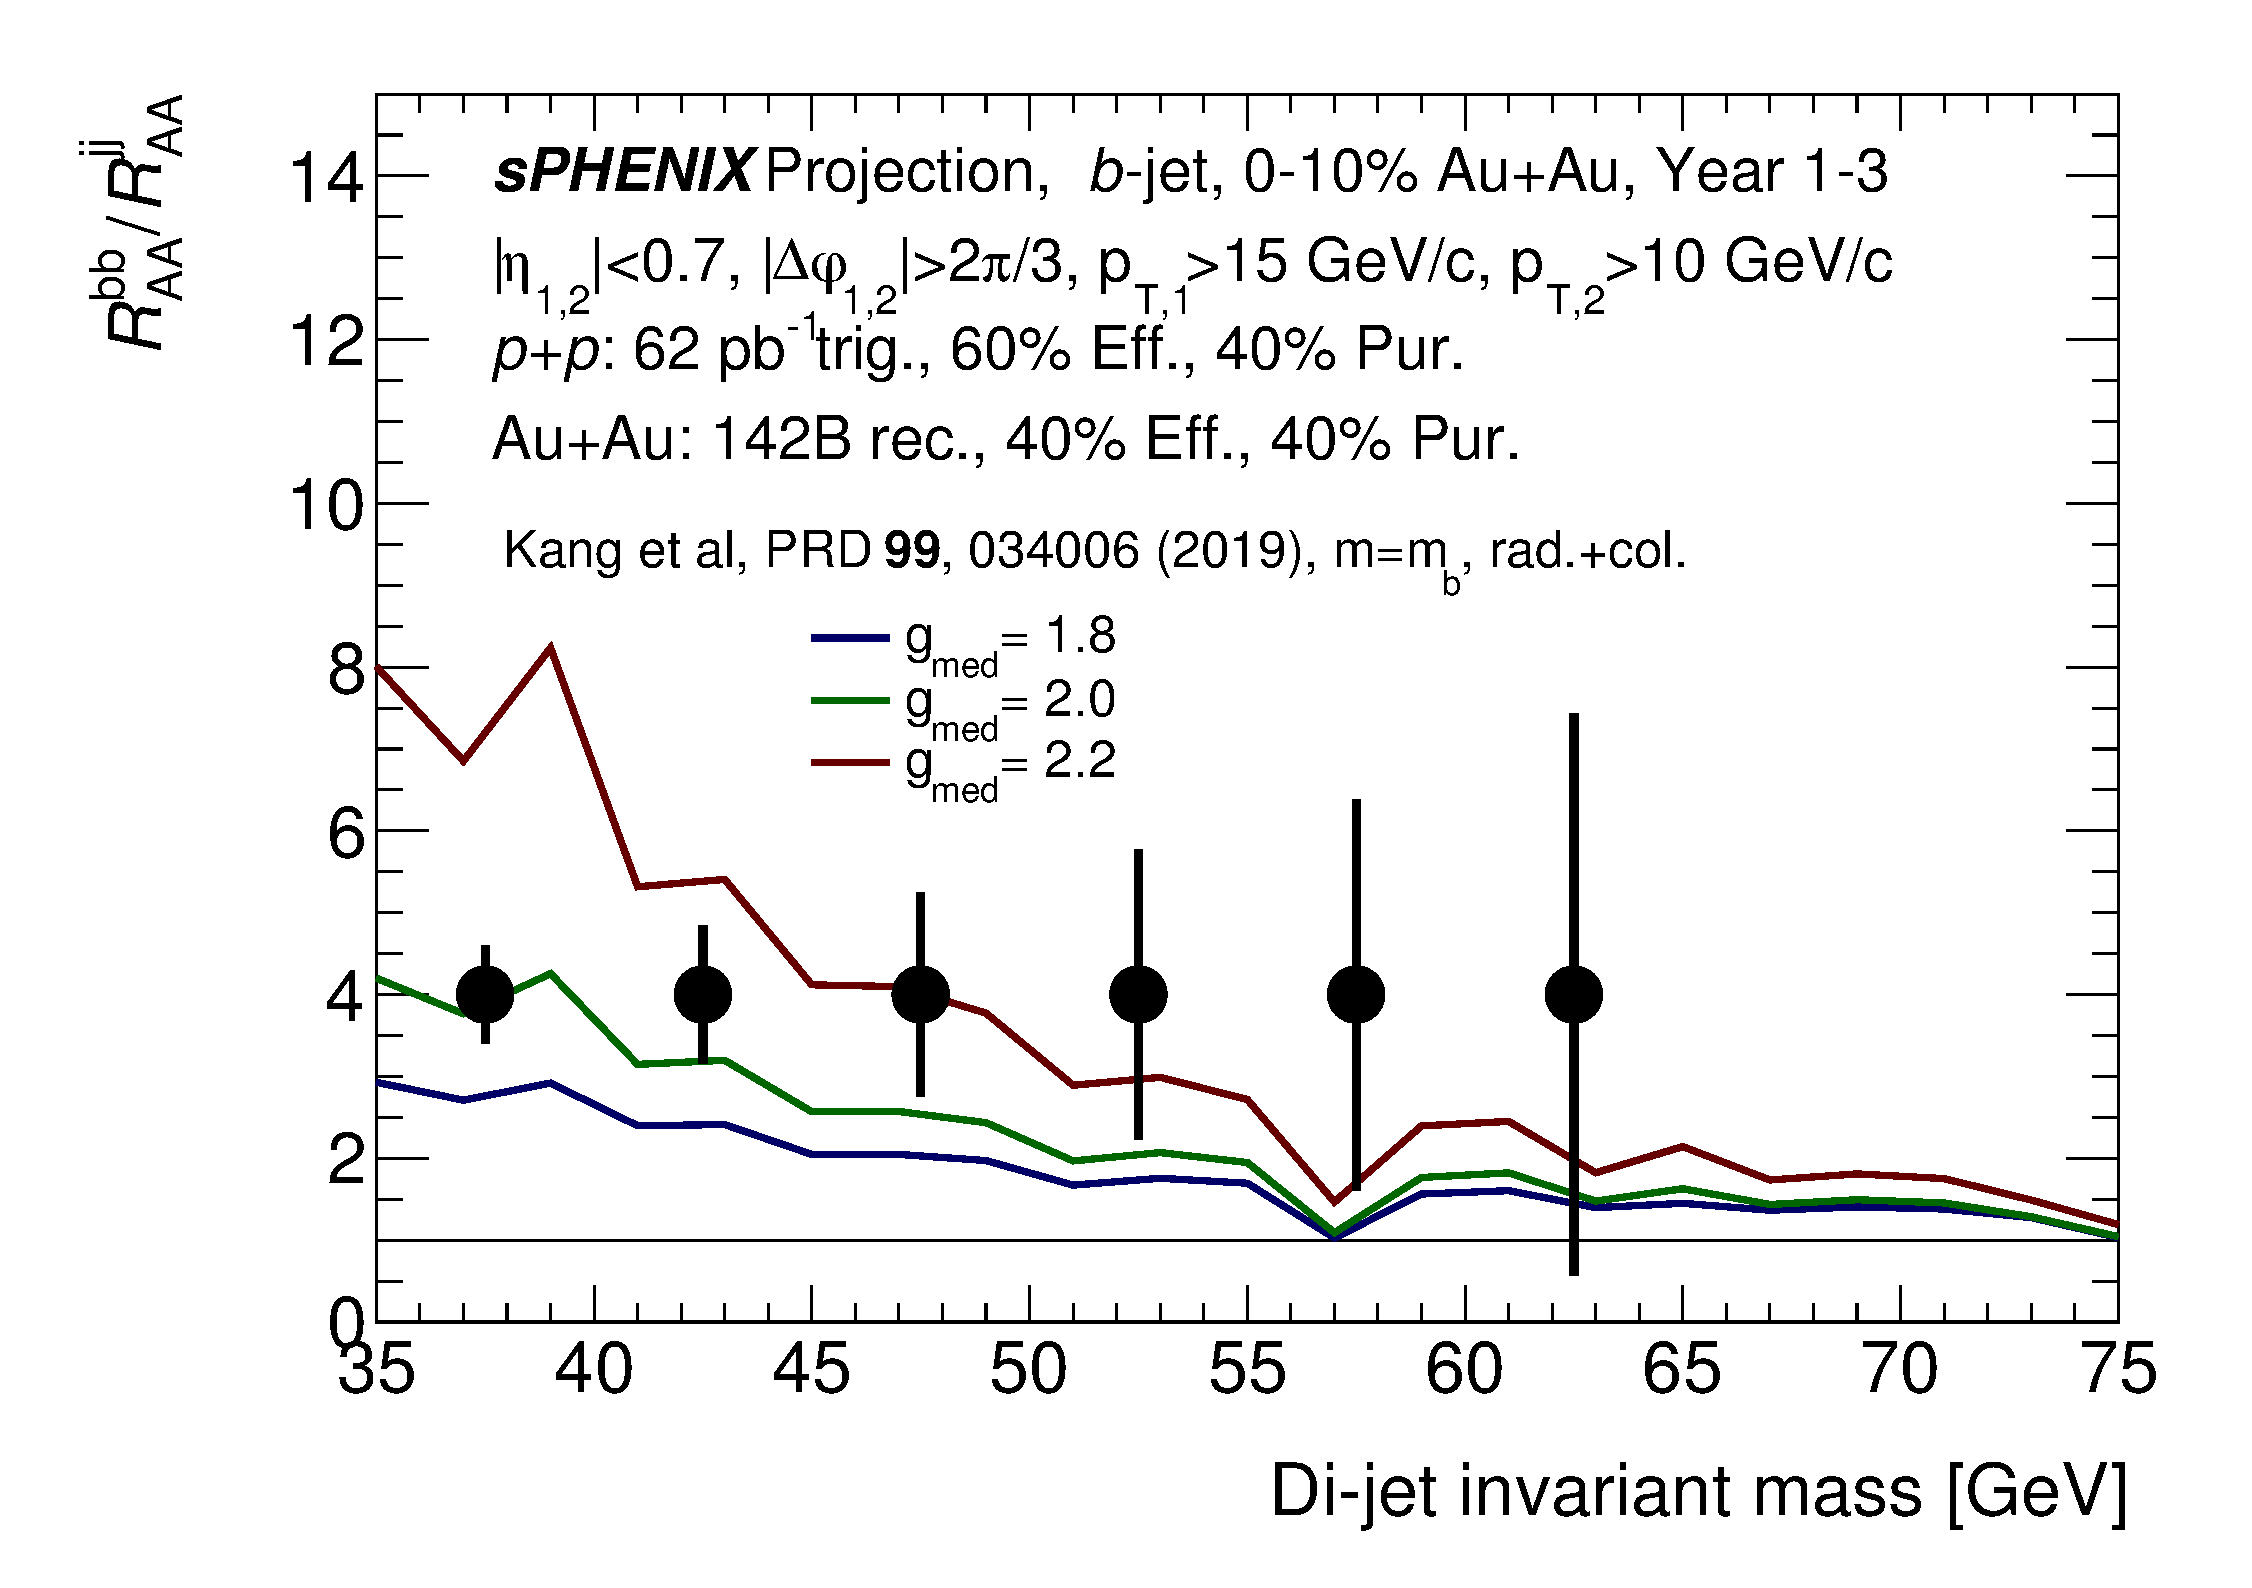
\includegraphics[width=0.48\textwidth]{figs/200pp_pythia8_CTEQ6L_7GeV_ALL_cfg_eneg_DSTReader_root_Draw_HFJetTruth_InvMass_CrossSection2RAARatio_Theory_3yr_deta0_70.pdf}
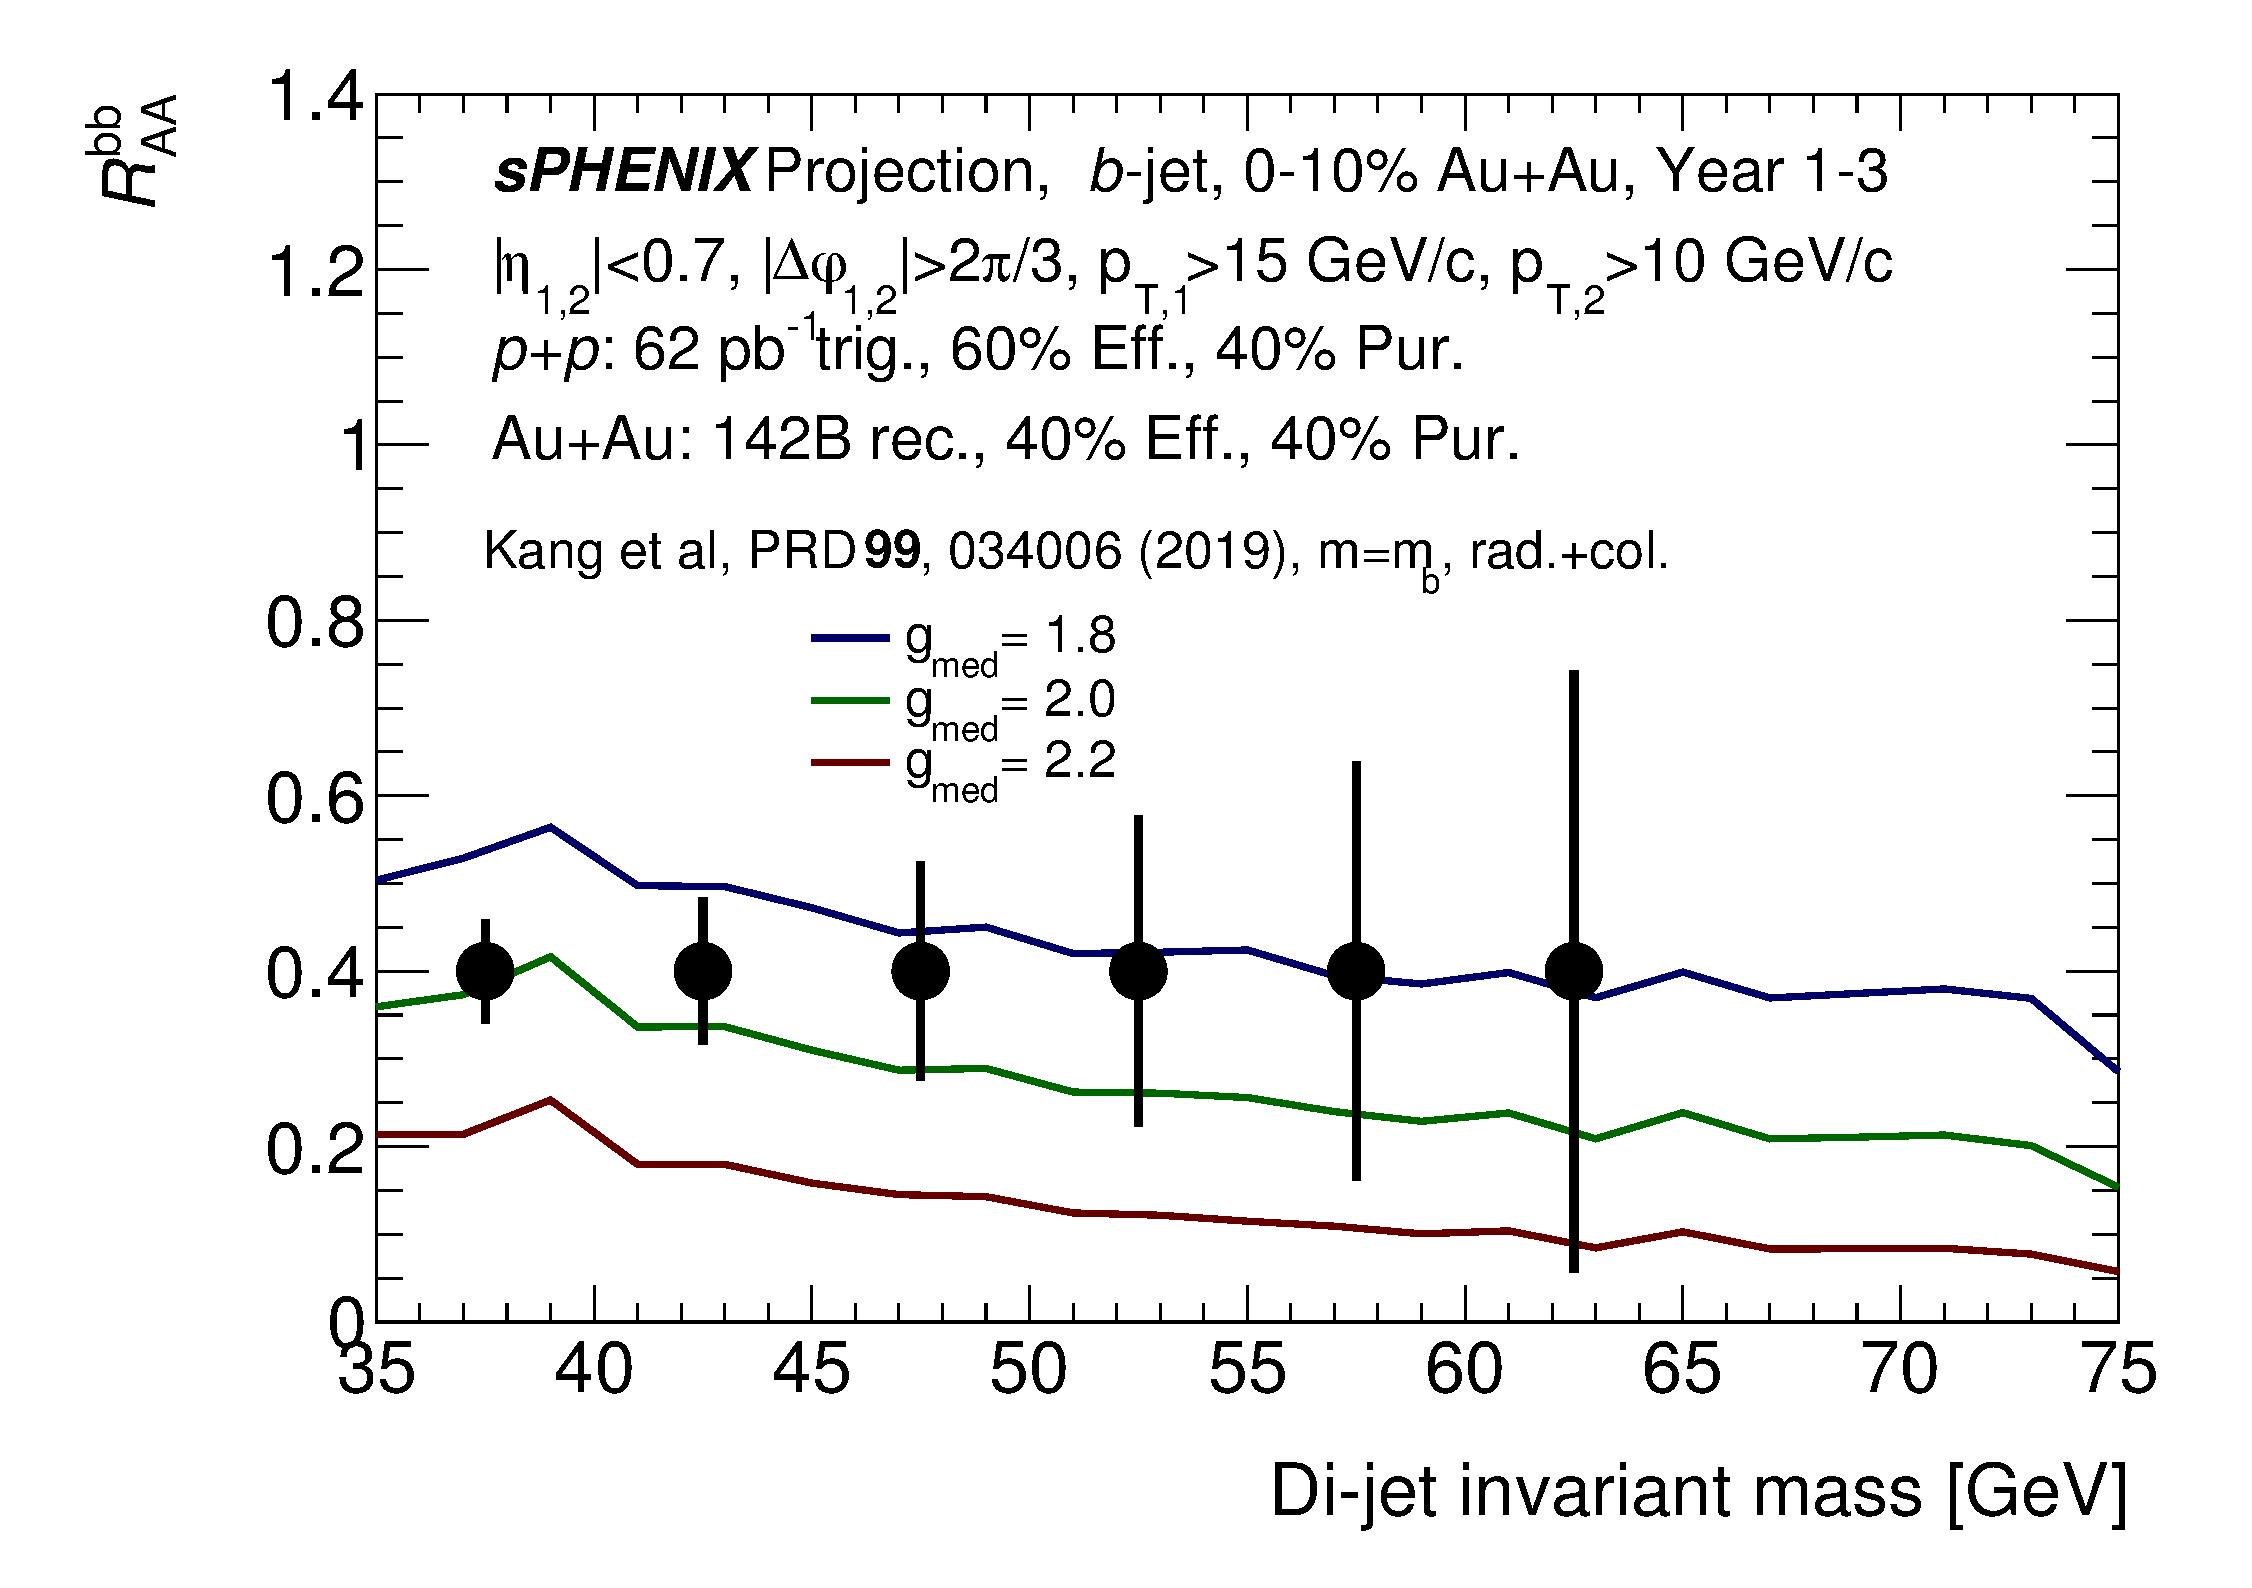
\includegraphics[width=0.5\textwidth]{figs/200pp_pythia8_CTEQ6L_7GeV_ALL_cfg_eneg_DSTReader_root_Draw_HFJetTruth_InvMass_CrossSection2RAA_Theory_3yr_deta0_70.pdf}
\caption{Projected statistical uncertainties of nuclear modification for $b$-jet pairs and $b$-jet-light-jet super-ratio.}
\label{fig:HF-bjet-pair}
\end{figure}



\begin{figure}[htbp]
\centering
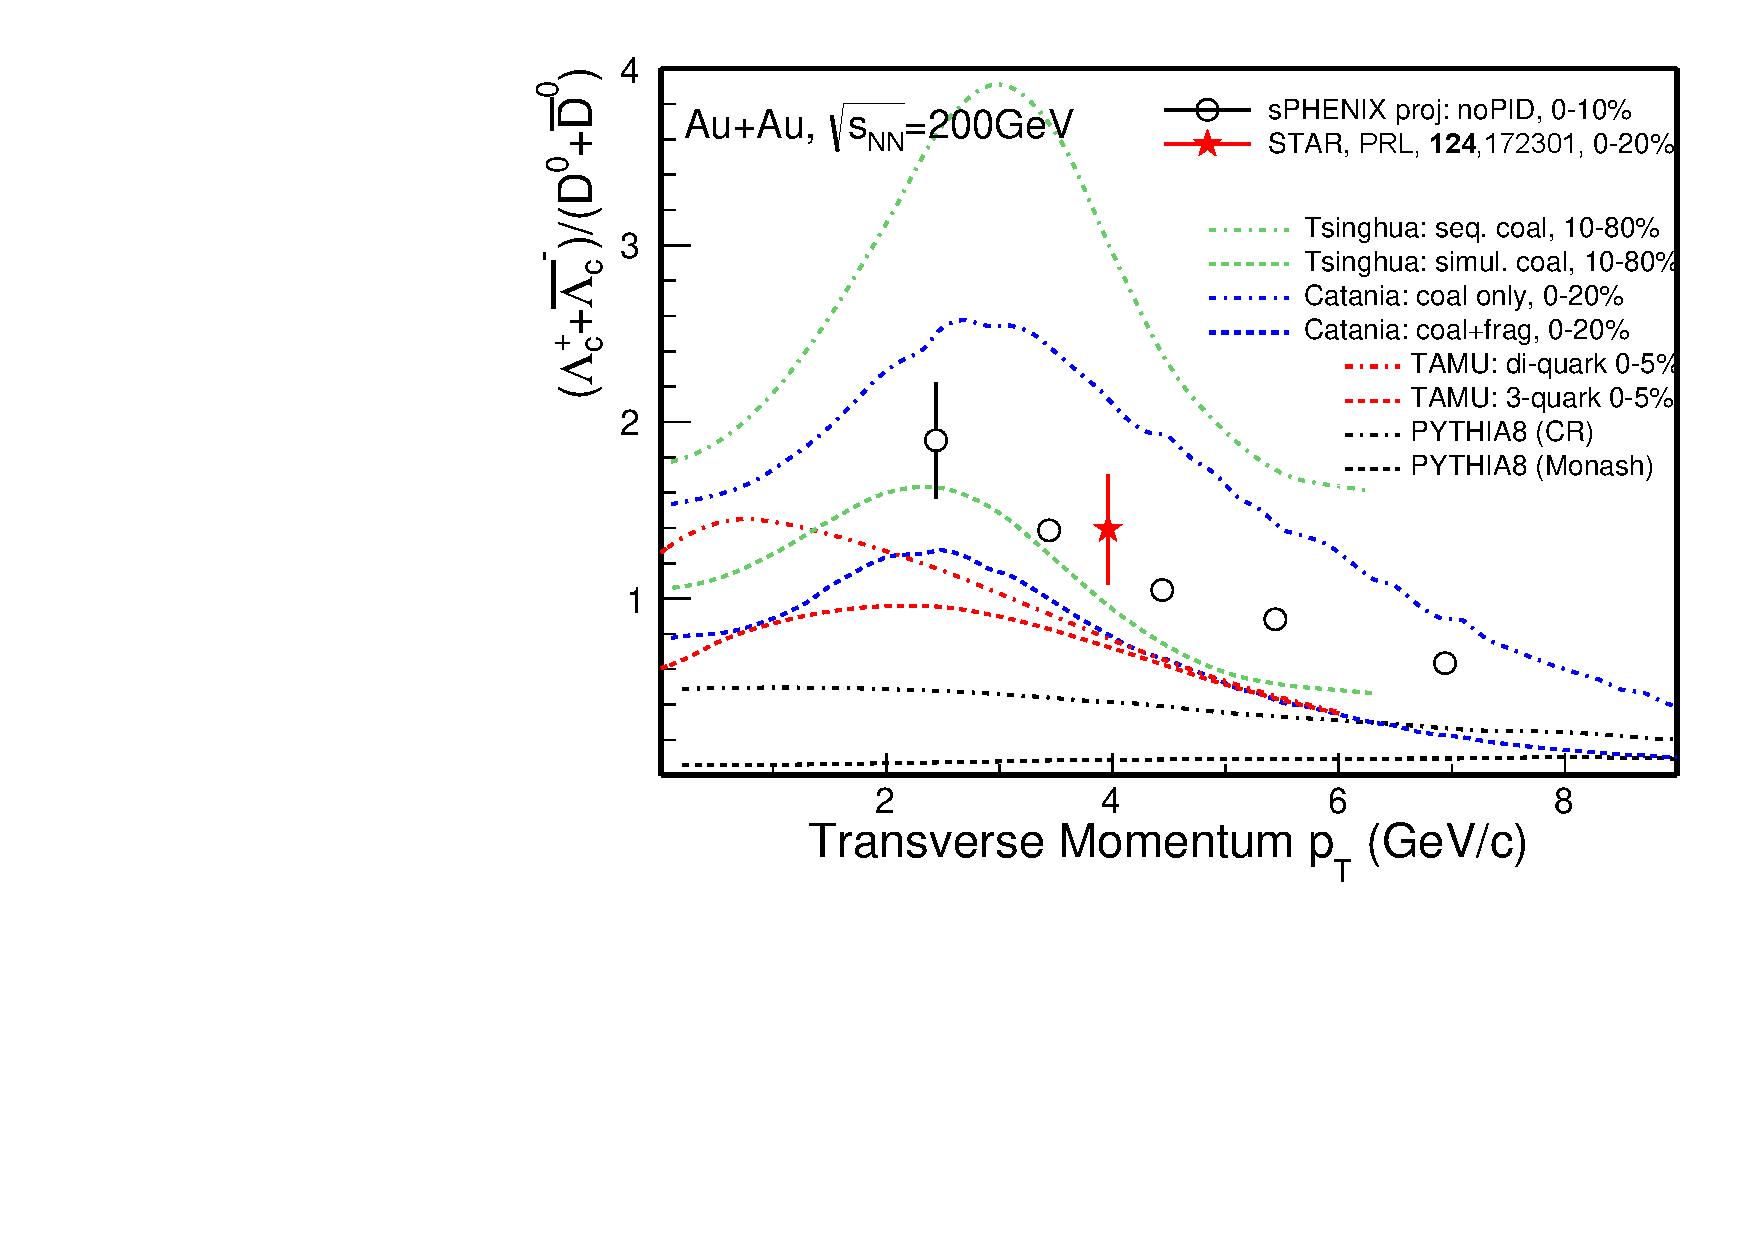
\includegraphics[width=0.48\textwidth]{figs/LcD0_proj_0_10_24B_Update.pdf}
\caption{Projected statistical uncertainties of $\lambda_c$ to $D^0$ ratio.}
\label{fig:HF-Lc}
\end{figure}



\section{Cold QCD Physics}
\label{sec:ColdQCD}

sPHENIX detector designed to study QGP with jet, photon and heavy flavor probes, with its trigger capabilities and high DAQ rate capabilities, will provide key opportunities for Cold QCD measurements. These include improving gluon polarization $\Delta G$ constraint at higher x utilizing longitudinally polarized beams, broad range of physics measurements with transversely polarized beams, and studies of transverse momentum effects and hadronization in $p+p$ and $p+A$ collisions.

The main emphasis of the RHIC Spin program has been measurements of the gluon polarization in longitudinally polarized proton collisions. RHIC experiments discovered a significant gluon polarization in the gluon momentum fraction range $x>0.05$. Even with the future EIC data expected to precisely measure $\Delta G$ in the lower x region, RHIC data will remain a significant contributor at $x>0.05$. However, any significant improvement of $\Delta G$ measurements, compared to existing RHIC data (published and being analyzed), requires significant integrated luminosity (at least a few hundred pb$^{-1}$), which is not anticipated in the sPHENIX 3-year running scenario. Therefore in this document we focus on the measurements with transversely polarized beams.

\subsection {Transverse Spin Measurements}

In recent years, transverse spin phenomena have gained substantial attention. The nature of significant transverse single spin asymmetry (TSSA) in hadron collisions, discovered more than 40 years ago at low center of mass energy $\sqrt{s}$=4.9 GeV, and then confirmed at higher energies, up to $\sqrt{s}$=500 GeV at RHIC, still remains not fully understood. Different mechanisms are suggested to explain such asymmetries, involving initial state and final state effects, in the collinear or transverse momentum dependent (TMD) framework. These descriptions have deep connections to nucleon partonic structure and parton dynamics within the nucleon.

TSSA in direct photon and heavy flavor production probe the gluon dynamics within the nucleon, described by tri-gluon correlation function in the collinear Twist-3 framework, which is connected with gluon Sivers function, at the moment poorly known. Sivers function correlates the nucleon transverse spin with the parton transverse
momentum. The projected uncertainties for direct photon TSSA compared to theoretical calculations are shown in Figure~\ref{fig:AN_dp} . The direct photon sample here will be collected with EMCal-based high energy cluster trigger. Asymmetry measurements in D0 meson production through its hadronic decay will be done from Minimum Bias sample collected with streaming readout. Figure~\ref{fig:AN-D0} shows the projected uncertainties for such a measurement.

\begin{figure}[htbp]
\centering
\includegraphics[width=0.60\textwidth]{figs/AN_dp_sphenix.pdf}
\caption{Projected statistical uncertainties for dir. photon $A_N$}
\label{fig:AN_dp}
\end{figure}

Another interesting channel related to Sivers effect is inclusive jet TSSA, not yet been measured at central rapidity. sPHENIX can provide high precision measurements with uncertainties on the level of a few times $10^{-4}$. While the opposite sign contribution of up and down quarks to Sivers asymmetry is expected to suppress the measured TSSA, tagging the leading hadron charge will "bias" the measurement towards the up or down quarks, and therefore will enables the flavor separated measurements in the central rapidity kinematics.

Di-jet measurements allows for direct access to parton intrinsic transverse momentum $k_T$. Again, charged tagging will allow to enhance the effect from either up or down quarks, which otherwise will be essentially cancelled out. Recent STAR preliminary results showed non-zero effect for charge tagged jets. sPHENIX as a dedicated detector for jet and photon measurements is expected to significantly contribute to these measurements and to extend it to photon-jet measurements, which essentially isolates quark-gluon scattering process, and therefore gives access to gluon Sivers effect.

Another possible origin of the TSSA is the Collins mechanism, which correlates the transverse polarization of a fragmented quark to the angular distribution of hadrons within a jet. This gives access to transversity distribution, which can be interpreted as the net transverse polarization of quarks within a transversely polarized proton. Along with unpolarized parton distribution function (PDF) and helicity PDF, transversity is one of three leading twist PDF, least known at the moment. The integral over the valence quark transversity defines tensor charge, a fundamental value calculable in lattice QCD, and therefore enabling the crucial comparison of experimental measurements with ab-initio theoretical calculations.

Measuring angular distributions of di-hadrons in the collisions of transversely polarized protons, couples transversity to the so-called “interference fragmentation function” (IFF) in the framework of collinear factorization. A comparison of the transversity signals extracted from the Collins effect and IFF measurements will explore questions about universality and factorization breaking. 

First non-zero Collins and IFF asymmetries in $p+p$ collisions has been observed by STAR collaboration, and shown to be invaluable to constrain transversity distribution. sPHENIX with its excellent hadron and jet calorimetric trigger capabilities coupled with its DAQ high rate capabilities, is expected to deliver high statistics samples for both Collins and IFF asymmetries. sPHENIX capability to collect a significant data sample with streaming readout will allow to extend the charged di-hadron measurements for IFF asymmetries from barrel region ($|\eta|<1$) to more forward kinematics up to $\eta=2$. Fig.* shows projected uncertainties for IFF asymmetries [hopefully we'll get them].

\subsection {Transverse Spin: pp vs pA}

$p\uparrow+A$ collisions at RHIC provide unique opportunities to study spin effects in nuclear environment. It may provide new insights into the origin of TSSA and a unique tool to investigate the rich phenomena behind TSSAs in hadronic collisions and to use TSSAs as a new approach to studying the small-system collisions.

First RHIC results from 2015 RHIC run showed a puzzling evolution of TSSA from $p+p$ to $p+Al$ and then $p+Au$. While STAR's preliminary result for $\pi^{0}$ asymmetry in forward rapidity (with $0.2<x_F<0.7$) showed no significant nuclear dependence, PHENIX positively charge hadron asymmetries in the intermediate rapidity range (with $0.1<x_F<0.2$) discovered a strong nuclear dependence in TSSA, from ~3\% in $p+p$ collisions to a value consistent with zero in $p+Au$ collisions. No clear explanation for such a behavior has been offered at the moment. Obviously, more data, differentiated in $p_T$ and $x_F$ would be highly desirable. sPHENIX is able to collect much more data in this channel, with fine binning, which is expected to provide crucial information on the nature of TSSA in hadronic collisions and on understanding of spin probe - nucleus interaction, a novel topic directly associated with RHIC unique ability to collide polarized protons with nuclei.

Fig.* showed the projected uncertainties for sPHENIX, based on MB data collected with the streaming readout. sPHENIX tracking system will provide us with charged hadron measurements in the pseudo-rapidity range up to $\eta=2$, which overlaps with the PHENIX range, where the strong nuclear effect was observed ($1.2<\eta<2.4$).

The other measurements (e.g. Collins and IFF asymmetries) will also be compared between $p+p$ and $p+A$ systems and may potentially bring new surprises.

\subsection {Unpolarized Measurements}

A number of cold QCD measurements, which don't require beam polarizations are planned in $p+p$ and $p+A$ collisions. Hadronization in a jet studies will be performed with hadron-in-jet measurements, multi-differential in momentum fraction z of the jet carried by the produced hadron and in $j_T$, the transverse momentum of the hadron with respect to the jet axis. This includes studies for both light quark and heavy quark hadrons. Comparison of $p+p$ and $p+A$ collisions will provide information on the nuclear modification of hadronization processes. Measurements of transverse momentum effects, and their nuclear modifications, in back-to-back di-hadron and photon-hadron correlations performed by PHENIX, will be extended to di-jet and photon-jet measurements in sPHENIX, which will help to separate the effects associated with intrinsic parton momentum $k_T$ and fragmentation transverse momentum $j_T$. Upsilon and J/$\Psi$ polarization measurements will shed further light on heavy quarkonium production mechanisms.

